\chapter{Vizualizacija podatkov}

\section{Knjižnica Matplotlib in njena namestitev}
Za vizualizacijo podatkov bomo uporabljali knjižnico Matplotlib, ki predstavlja osnovo za risanje kakršnihkoli grafov. Ker v osnovni različici jezika Python še ni nameščen, ga moramo pred uporabo namestiti (če imate nameščeno distribucijo Anaconda, imate to knjižnico že nameščeno). Kot smo spoznali v poglavju \ref{ch:moduli} lahko za namestitev knjižnice uporabimo orodje \texttt{pip}, tako da zaženemo ukazno vrstico svojega operacijskega sistema (ne okolja IDLE) in vanjo vpišemo
\begin{lstlisting}[language=bash]
> pip install matplotlib
\end{lstlisting}
Podrobnejša navodila za namestitev paketov smo podali že v poglavju \ref{ch:moduli}, zato jih tu ne bomo podvajali. Če ima vaš računalnik povezavo z internetom, bo orodje \texttt{pip} samo preneslo potrebne namestitvene datoteke in knjižnico namestilo.

Za vizualizacija naših podatkov bomo uporabili Matplotlibov vmesnik \angl{interface} \texttt{pyplot}, ki nam risanje precej olajša. V svoje programe ga bomo uvozili takole:
\begin{lstlisting}[language=Python, showstringspaces=false]
import matplotlib.pyplot as plt
\end{lstlisting}
Zdaj lahko do funkcij za risanje grafov dostopamo takole:
\begin{lstlisting}[language=Python, showstringspaces=false]
plt.ime_funkcije(argumenti)
\end{lstlisting}

\section{Funkciji \texttt{plot} in \texttt{show}}

Začeli bomo s funkcijo \texttt{plot}, ki omogoča izris črtnega grafa \angl{line plot}. V osnovi ji lahko podamo zgolj en seznam. Poskusimo:
\begin{lstlisting}[language=Python, showstringspaces=false]
>>> Y = [1, 3, 9, 12]
>>> plt.plot(Y)
[<matplotlib.lines.Line2D object at 0x000001DD7FB28860>]
\end{lstlisting}
Nekaj se je očitno zgodilo, grafa pa še vedno ne vidimo. Funkcija \texttt{plot} namreč deluje tako, da grafe riše v ozadju in te dodaja na risalno površino, ki pa jo pokaže, šele ko pokličemo funkcijo \texttt{show}.
\begin{lstlisting}[language=Python, showstringspaces=false]
>>> plt.show()
\end{lstlisting}
Zdaj se je pokazal graf, ki ga prikazuje slika \ref{img:plt1}.
\begin{figure}
    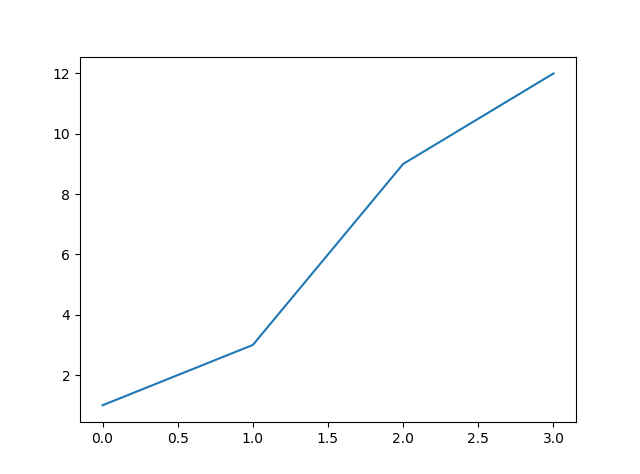
\includegraphics[width=\linewidth]{img/plt1.png}
    \caption{Črtni graf, pri čemer smo podali koordinate točk na osi $y$.}
    \label{img:plt1}
\end{figure}
Točke, ki smo jih podali funkciji \texttt{plot}, očitno predstavljajo koordinate $y$ narisanega grafa. Točke na osi $x$ je Matplotlib določil kar glede na indekse točke v seznamu \texttt{Y}. To lahko spremenimo, tako da funkcijo \texttt{plot} pokličemo z dvema seznamoma, pri čemer prvi določa koordinate točk na osi $x$ drugi pa koordinate točk na osi $y$. Seznama morata biti seveda enakih dolžin. Do enakega grafa kot zgoraj, bi lahko prišli takole: 
\begin{lstlisting}[language=Python, showstringspaces=false]
>>> Y = [1, 3, 9, 12]
>>> X = range(len(Y))
>>> plt.plot(X, Y)
[<matplotlib.lines.Line2D object at 0x000002042BEBC128>]
plt.show()
\end{lstlisting}
Os $x$ bi lahko tudi spremenili. Poskusimo:
\begin{lstlisting}[language=Python, showstringspaces=false]
>>> X = [1,3,4,5]
>>> Y = [1, 3, 9, 12]
>>> plt.plot(X,Y)
[<matplotlib.lines.Line2D object at 0x000002042A9D0DA0>]
>>> plt.show()
\end{lstlisting}
Graf, ki smo ga narisali tako, prikazuje slika \ref{img:plt2}.
\begin{figure}
    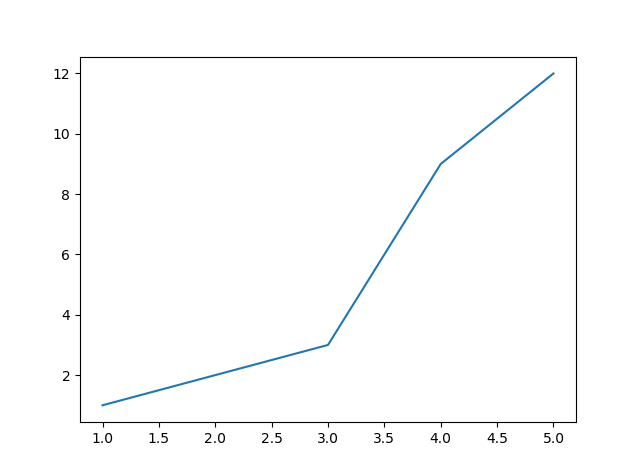
\includegraphics[width=\linewidth]{img/plt2.png}
    \caption{Črtni graf, pri čemer smo podali koordinate točk na obeh oseh.}
    \label{img:plt2}
\end{figure}
Na sliki je prikazan samo zadnji graf. Kam je izginil prejšnji? Kot smo že omenili knjižnica Matplotlib grafe riše na risalni površini v ozadju. Te prikaže, ko pokličemo funkcijo \texttt{show}, hkrati pa takrat risalno površino tudi počisti. Če hočemo na isti sliki prikazati več grafov, bomo pred klicanjem funkcije \texttt{show} pač narisali več grafov. Poskusimo to kar na zgledu s plačami. Predpostavljali bomo, da smo funkcijo \texttt{uvozi\_place} shranili v program \texttt{place\_beri.py} in da se ta program nahaja v naši trenutni delovni mapi. Najprej bomo uvozili funkcijo za uvoz podatkov o plačah zraven pa še knjižnico Matplotlib:
\begin{lstlisting}[language=Python, showstringspaces=false]
>>> from place_beri import uvozi_place
>>> import matplotlib.pyplot as plt
\end{lstlisting}
Potem preberimo podatke o plačah:
\begin{lstlisting}[language=Python, showstringspaces=false]
>>> MJ, ZJ, MZ, ZZ = uvozi_place('place.csv')
\end{lstlisting}
Zdaj bomo kot koordinate na osi $x$ podali podatke o mesecih, kot koordinate na osi $y$ pa podatke o zneskih in poklicali funkcijo za prikaz grafa. Takole:
\begin{lstlisting}[language=Python, showstringspaces=false]
>>> plt.plot(MJ, ZJ)
>>> plt.plot(MZ, ZZ)
>>> plt.show()
\end{lstlisting}
Več grafov lahko na isto sliko narišemo tudi tako, da naštejemo pare seznamov kar po vrsti. Takole: 
\begin{lstlisting}[language=Python, showstringspaces=false]
>>> plt.plot(MJ, ZJ, MZ, ZZ)
>>> plt.show()
\end{lstlisting}
Kljub temu, da je rezultat v zgornjih dveh primerih enak, bomo raje uporabljali prvi način.
Zapišimo zdaj vse skupaj kot program \texttt{risi\_place.py}.
\begin{lstlisting}[language=Python, showstringspaces=false,numbers=left]
from place_beri import uvozi_place # funkcija za uvoz
import matplotlib.pyplot as plt 
MJ, ZJ, MZ, ZZ = uvozi_place('place.csv')
plt.plot(MJ, ZJ) # riši javni sektor
plt.plot(MZ, ZZ) # riši zasebni sektor
plt.show() # prikaži graf
\end{lstlisting}
Rezultat izvedbe zgornjega programa prikazuje slika \ref{img:plt3}.
\begin{figure}
    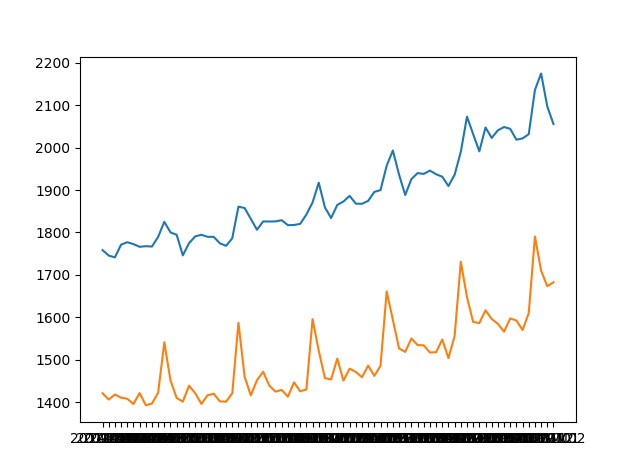
\includegraphics[width=\linewidth]{img/plt3.png}
    \caption{Osnovni izris podatkov o plačah.}
    \label{img:plt3}
\end{figure}

\section{Dodajanje oznak}
Vsak graf seveda potrebuje oznake. Označiti moramo kaj prikazuje posamezna os, za kar lahko uporabimo funkciji \texttt{xlabel} in \texttt{ylabel}, ki kot argument prejmeta niz, ki ga želimo prikazati. V našem primeru bi bilo smiselno napisati takole:
\begin{lstlisting}[language=Python, showstringspaces=false]
plt.xlabel("mesec")
plt.ylabel("znesek [EUR]")
\end{lstlisting}
Dodamo lahko tudi naslov grafa z uporabo funkcije \texttt{title}. Takole:
\begin{lstlisting}[language=Python, showstringspaces=false]
plt.title("Povprečne mesečne plače")
\end{lstlisting}

Manjka seveda tudi legenda. Kaj prikazuje modra linija in kaj oranžna? Legendo lahko dodamo tako, da oznake dodamo še posameznemu grafu kar med izrisom. Funkciji \texttt{plot} lahko preko opcijskega argumenta \texttt{label} podamo niz, ki predstavlja oznako grafa, ki ga bo izrisala. V našem primeru bi to naredili takole:
\begin{lstlisting}[language=Python, showstringspaces=false]
plt.plot(MJ, ZJ, label='javni') # riši javni sektor
plt.plot(MZ, ZZ, label='zasebni') # riši zasebni sektor
\end{lstlisting}
Če želimo legendo pokazati, moramo poklicati še funkcijo \texttt{legend}, ki prikaz legende vklopi:
\begin{lstlisting}[language=Python, showstringspaces=false]
plt.legend()
\end{lstlisting}
Vsebino legende, ki jo želimo izpisati bi lahko podali tudi neposredno funkciji \texttt{legend}. Takole:
\begin{lstlisting}[language=Python, showstringspaces=false]
plt.legend(['javni', 'zasebni'])
\end{lstlisting}
Pri tem moramo paziti na to, da oznake v legendi podajamo v enakem vrstnem redu, kot smo izvajali risanje grafov.


Zapišimo celoten program, ga poženimo in poglejmo rezultat. 
\begin{lstlisting}[language=Python, showstringspaces=false,numbers=left]
from place_beri import uvozi_place # funkcija za uvoz
import matplotlib.pyplot as plt

MJ, ZJ, MZ, ZZ = uvozi_place('place.csv')
plt.plot(MJ, ZJ) # riši javni sektor
plt.plot(MZ, ZZ) # riši zasebni sektor

# dodaj oznake
plt.xlabel("mesec")
plt.ylabel("znesek [EUR]")
plt.title("Povprečne mesečne plače")
plt.legend(['javni', 'zasebni'])

plt.show() # prikaži graf
\end{lstlisting}
Rezultat izvedbe zgornjega programa prikazuje slika \ref{img:plt4}.
\begin{figure}
    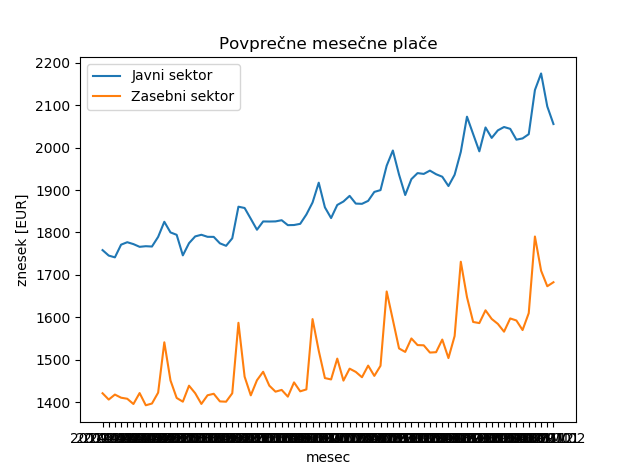
\includegraphics[width=\linewidth]{img/plt4.png}
    \caption{Izris podatkov o plačah z dodanimi oznakami.}
    \label{img:plt4}
\end{figure}

\section{Še malo prilagajanja oznak}
Kar nam še vedno ni všeč na sliki \ref{img:plt4} je neberljiv izpis na osi $x$. Če graf približamo, vidimo, da je na oseh izpisan podatek o mesecu. Mogoče bi bilo bolje, če bi ta podatek izpisali samo vsak januar, poleg tega pa bi informacijo o mesecu izpustili. Poskusimo odrezati rezino po mesecih od začetka do konca, pri čemer za korak nastavimo vrednost 12.
\begin{lstlisting}[language=Python, showstringspaces=false]
>>> MJ[::12]
['2014M01', '2015M01', '2016M01', '2017M01', '2018M01',
'2019M01', '2020M01']
\end{lstlisting}
Pripravimo si seznam \texttt{oznake}, ki bo vseboval samo podatke o letih. Vzeli bomo vsak 12-ti podatek iz obstoječega seznama mesecev (izhajamo lahko bodisi is seznama \texttt{MJ} ali \texttt{MZ}), pri čemer bomo upoštevali samo prve štiri znake (podatek o letu). 
\begin{lstlisting}[language=Python, showstringspaces=false]
oznake = []
for mj in MJ[::12]: # vzamemo vsako 12-to oznako
    oznake.append(mj[:4]) # vzamemo samo podatek o letu
\end{lstlisting}
Določiti moramo še lokacije, kjer bomo te oznake prikazali. Trenutno so oznake prikazane na lokacijah, ki se ujemajo z njihovimi indeksi, torej bi lahko lokacije oznak dobili s seznamoma \texttt{range(len(MJ))} ter \texttt{range(len(MZ))}. Ker bi radi prikazali vsako 12-to oznako, bomo morali torej upoštevati tudi vsako 12-to lokacijo. Takole:
\begin{lstlisting}[language=Python, showstringspaces=false]
# vsaka 12-ta lokacija
lokacije = range(0, len(MJ), 12) 
\end{lstlisting}

Lokacijo in vsebino oznak lahko zdaj našemu risarju podamo preko funkcije \texttt{xticks} (če bi želeli prilagajati oznake na osi $y$, bi uporabili funkcijo \texttt{yticks}):
\begin{lstlisting}[language=Python, showstringspaces=false]
plt.xticks(lokacije, oznake)
\end{lstlisting}

Celoten program je zdaj sledeč:
\begin{lstlisting}[language=Python, showstringspaces=false,numbers=left]
from place_beri import uvozi_place # funkcija za uvoz
import matplotlib.pyplot as plt

MJ, ZJ, MZ, ZZ = uvozi_place('place.csv')
plt.plot(MJ, ZJ) # riši javni sektor
plt.plot(MZ, ZZ) # riši zasebni sektor

# dodaj oznake
plt.xlabel("mesec")
plt.ylabel("znesek [EUR]")
plt.title("Povprečne mesečne plače")
plt.legend(['javni', 'zasebni'])

oznake = []
for mj in MJ[::12]: # vzamemo vsako 12-to oznako
    oznake.append(mj[:4]) # vzamemo samo podatek o letu

# vsaka 12-ta lokacija
lokacije = range(0, len(MJ), 12) 

plt.xticks(lokacije, oznake)

plt.show() # prikaži graf
\end{lstlisting}
Rezultat izvedbe programa prikazuje slika \ref{img:plt5}.
\begin{figure}
    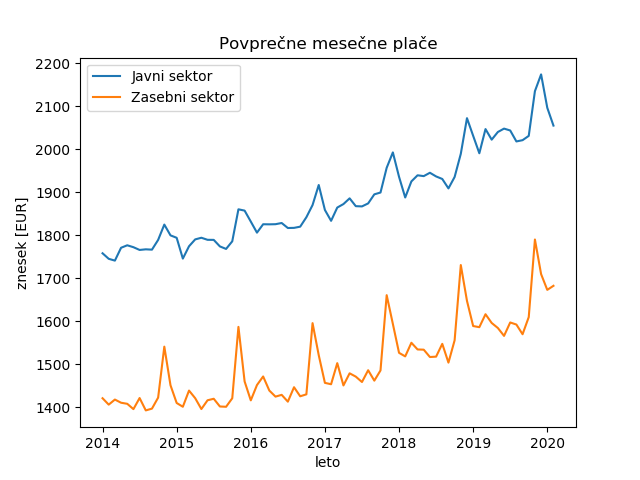
\includegraphics[width=\linewidth]{img/plt5.png}
    \caption{Izris podatkov o plačah s prilagojenimi oznakami na osi $x$.}
    \label{img:plt5}
\end{figure}

\section{Ostale prilagoditve izrisa}
Če nam grafi še vedno niso všeč, se lahko igramo naprej. Preko funkcije \texttt{plot} lahko nastavljamo barvo izrisa (argument \texttt{color}), debelino črte (argument \texttt{linewidth}), tip črte (argument \texttt{linestyle}) in še marsikaj. Poleg tega lahko določamo razpon osi (funkcija \texttt{axis}), rišemo več podgrafov (funkcija \texttt{subplot}) in graf shranjujemo v datoteko (funkcija \texttt{savefig}). Možnosti je res veliko in jih tukaj ne bomo več naštevali. Primere različnih grafov, ki jih lahko izrišemo z uporabo knjižnice Matplotlib, si lahko bralec pogleda (in prosto dostopno kodo prilagodi za risanje svojih grafov) na povezavi \url{https://matplotlib.org/gallery}.

\section{Ostali tipi grafov}

Matplotlib poleg črtnega diagrama (funkcija \texttt{plot})

\section{Risanje matematičnih funkcij}
